\documentclass{article}
\usepackage[utf8]{inputenc}
\usepackage[brazilian]{babel}
\usepackage{url}
\usepackage{graphicx}
\usepackage{geometry}
\usepackage{enumitem}
\usepackage{float}
\usepackage{amsmath}
\usepackage[table,xcdraw]{xcolor}
\usepackage{multirow}
\usepackage{caption}

\geometry{a4paper, left=20mm, right=20mm, top=20mm, bottom=20mm}
 

\begin{document}

  \begin{frame}{}
      \hspace*{-0.5cm}
      $\vcenter{\hbox{
\includegraphics[width=1cm]{mackenzie-logo.png}}}$
      $\vcenter{\resizebox{0.95\textwidth}{!}{
          \begin{tabular}{c}
            Leandro N. de Castro \& Daniel Ferrari  \\
            Introdução à Mineração de Dados: Conceitos Básicos, Algoritmos e Aplicações \\
              \hline 
              Marcos Cordeiro de Brito Jr
          \end{tabular}
      }}$
  \end{frame}

  \begin{center}
    \huge \textbf{CADERNO DE EXERCÍCIOS – PARTE 02} \\ 
  \end{center}

  \setcounter{section}{3}
  \section{CAPÍTULO 04: AGRUPAMENTO DE DADOS}
  \subsection{EXERCÍCIOS CONCEITUAIS}
  \subsubsection{Qual é a definição e o objetivo da tarefa de agrupamento de dados?}
  \textit{Resposta:} A tarefa de agrupamento de dados tem por objetivo descobrir grupos homogêneos de objetos utilizando métodos numéricos de análise de dados multivariados. \\
  Ela pode ser definida como a organização de um conjunto de objetos, normalmente representados por pontos em um espaço multidimensional em grupos baseada na similaridade entre eles. 


  \subsubsection{A avaliação da saída de um algoritmo de agrupamento de dados pode determinar a qua-lidade do agrupamento resultante. Para isso utilizamos medidas de avaliação de desem-penho que são responsáveis por aferir quantitativamente o agrupamento resultante. As medidas podem ser categorizadas em dois tipos. Quais são os tipos de medidas de avaliação e como eles funcionam?}
  \textit{Resposta:} Os dois tipos de medidas são: internas e externas.
  \begin{itemize}
    \item \textbf{Internas:} são medidas que utilizam apenas informações intrínsecas aos objetos do agrupamento baseando-se em medidas de similaridade e avaliando as distâncias intragrupos e/ou intergrupos.
    
    \item  \textbf{Externas:} são medidas que avaliam quão correto está um agrupamento dado um agrupamento ideal que se deseja alcançar. O cálculo dessas medidas requer o conhecimento prévio do grupo ao qual cada objeto pertence. 

  \end{itemize}


  \subsubsection{Existem diversos algoritmos de agrupamento disponíveis, mas de forma abrangente estes algoritmos podem ser divididos em três categorias. Quais são estas categorias e suas características?}
  \textit{Resposta:} As três categorias são: hierárquicos, particionais e não exclusivos.
  Abaixo estão as características de cada um.
  \begin{itemize}
    \item \textbf{Hierárquicos:} os métodos hierárquicos criam uma decomposição hierárquica dos dados. Esses métodos podem ser aglomerativos ou divisivos, baseados em como o processo de decomposição é efetuado. 

    \item \textbf{Particionais:} a partir de um número $n$ de partições, o método constrói $k$ partições dos dados, sendo cada partição representa um cluster onde $k \leq n$.  

    \item \textbf{Não Exclusivos:} esse método permite que um objeto pertença completamente ou parcialmente a mais de um grupo ao mesmo tempo.
  \end{itemize}
  \newpage

  \subsection{EXERCÍCIOS NUMÉRICOS}

  \subsubsection{Para a base de dados apresentada na tabela abaixo execute dois passos do algoritmo $k$-Médias, com $k = 2$ e distância Euclidiana. Considere os objetos 1 e 4 como centroides iniciais.}
  \begin{figure}[H]
      \centering 
      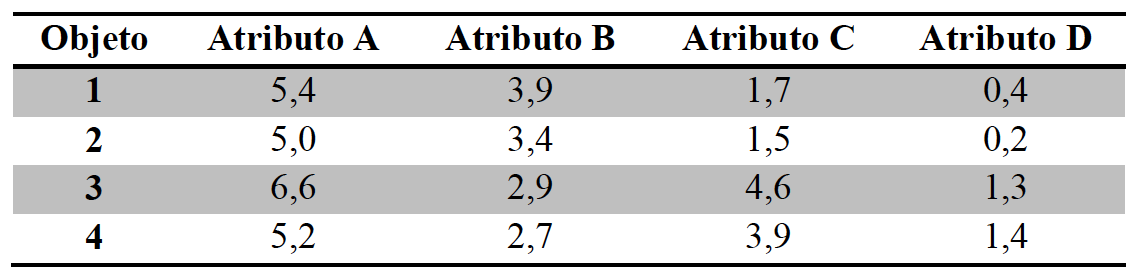
\includegraphics[width=12cm]{tab-4-2-1.png} 
    \end{figure}

  \textit{Resposta:} \\
  \textbf{Centroides}

  \begin{table}[H]
    \centering
    \begin{tabular}{|c|c|c|c|c|c|c|}
    \hline
    \rowcolor[HTML]{EFEFEF} 
    \textbf{Cluster} & \textbf{Objeto} & \textbf{Atributo A} & \textbf{Atributo B} & \textbf{Atributo C} & \textbf{Atributo D} & \textbf{Centroides}  \\ \hline
    C1               & 1               & 5.4                 & 3.9                 & 1.7                 & 0.4                 & (5.4, 3.9, 1.7, 0.4) \\ \hline
    C2               & 4               & 5.2                 & 2.7                 & 3.9                 & 1.4                 & (5.2, 2.7, 3.9, 1.4) \\ \hline
    \end{tabular}
  \end{table}

  \begin{table}[H]
    \centering
    \begin{tabular}{|c|c|}
    \hline
    \rowcolor[HTML]{EFEFEF} 
    \textbf{Cluster} & \textbf{Centroides}  \\ \hline
    C1               & (5.4, 3.9, 1.7, 0.4) \\ \hline
    C2               & (5.2, 2.7, 3.9, 1.4) \\ \hline
    \end{tabular}
  \end{table}

  \textbf{Iteração 1}

  \begin{table}[H]
    \centering
    \begin{tabular}{|c|c|c|c|c|}
    \hline
    \rowcolor[HTML]{EFEFEF} 
    \textbf{Objeto} & \textbf{Atributo A} & \textbf{Atributo B} & \textbf{Atributo C} & \textbf{Atributo D} \\ \hline
    2               & 5.0                 & 3.4                 & 1.5                 & 0.2                 \\ \hline
    \end{tabular}
  \end{table}

  \begin{center}
    $d(x_2,c_1) = \sqrt{(5.0 - 5.4)^2 + (3.4 - 3.9)^2 + (1.5 - 1.7)^2 + (0.2 - 0.4)^2} $  \\
    $d(x_2,c_1) = \sqrt{0.16 + 0.25 + 0.04 + 0.16} $  \\
    $d(x_2,c_1) = \sqrt{0.61} $ \\ 
    $d(x_2,c_1) = \textbf{0.78} $ \\
  \end{center}

  \begin{center}
    $d(x_2, c_2) =  \sqrt{(5.0 - 5.2)^2 + (3.4 - 2.7)^2 + (1.5 - 3.9)^2 + (0.2 - 1.4)^2} $ \\
    $d(x_2, c_2) = \sqrt{ 0.4 + 0.49 +  5.76 + 1.44}$
    $d(x_2,c_1) = \sqrt{8.09} $ \\
    $d(x_2,c_1) =  2.84 $\\
  \end{center}

  \begin{table}[H]
    \centering
    \begin{tabular}{|c|c|}
    \hline
    \rowcolor[HTML]{EFEFEF} 
    \textbf{Objeto} & \textbf{Cluster} \\ \hline
    1               & C1               \\ \hline
    2               & C1               \\ \hline
    3               &                  \\ \hline
    4               & C2               \\ \hline
    \end{tabular}
  \end{table}

  \textbf{Recalculando Centroide C1}
  \newline
  \textbf{Atual}
  \begin{table}[H]
    \centering
    \begin{tabular}{|c|c|c|c|c|c|c|}
    \hline
    \rowcolor[HTML]{EFEFEF} 
    \textbf{Cluster} & \textbf{Objeto} & \textbf{Atributo A} & \textbf{Atributo B} & \textbf{Atributo C} & \textbf{Atributo D} & \textbf{Centroides}  \\ \hline
    C1               & 1               & 5.4                 & 3.9                 & 1.7                 & 0.4                 & (5.4, 3.9, 1.7, 0.4) \\ \hline
    \end{tabular}
  \end{table}
  \textbf{Novo}
  \begin{center}
    $C_1 = (\dfrac{5.4+5.0}{2}, \dfrac{3.9+3.4}{2}, \dfrac{1.7+1.5}{2}, \dfrac{0.4+0.2}{2})$ \\
    $C_1 = (5.2, 3.65, 1.6, 0.3)$

    \begin{table}[H]
      \centering
      \begin{tabular}{|c|c|}
      \hline
      \rowcolor[HTML]{EFEFEF} 
      \textbf{Cluster} & \textbf{Centroides}  \\ \hline
      C1               & (5.2,3.65,1.6,0.3)   \\ \hline
      C2               & (5.2, 2.7, 3.9, 1.4) \\ \hline
      \end{tabular}
    \end{table}
  \end{center}


  \textbf{Iteração 2}

  \begin{table}[H]
    \centering
    \begin{tabular}{|c|c|c|c|c|}
    \hline
    \rowcolor[HTML]{EFEFEF} 
    \textbf{Objeto} & \textbf{Atributo A} & \textbf{Atributo B} & \textbf{Atributo C} & \textbf{Atributo D} \\ \hline
    3               & 6.6                 & 2.9                 & 4.6                 & 1.3                 \\ \hline
    \end{tabular}
  \end{table}

  \begin{center}
    $d(x_3,c_1) = \sqrt{(6.6-5.2)^2 + (2.9-3.65)^2 + (4.6-1.6)^2 +(1.3-0.3)^2}$  \\
    $d(x_3,c_1) = \sqrt{1.96 + 0.56 + 9 + 1}$ \\
    $d(x_3,c_1) = \sqrt{12.52}$ \\
    $d(x_3,c_1) = 3.54$
  \end{center}

  \begin{center}
    $d(x_3,c_2) = \sqrt{(6.6-5.2)^2 + (2.9-2.7)^2 + (4.6-3.9)^2 +(1.3-1.4)^2}$  \\
    $d(x_3,c_2) = \sqrt{1.96 + 0.04 + 0.49 + 0.01}$ \\
    $d(x_3,c_2) = \sqrt{2.5}$ \\
    $d(x_3,c_2) = \textbf{1.58}$
  \end{center}

  \begin{table}[H]
    \centering
    \begin{tabular}{|c|c|}
    \hline
    \rowcolor[HTML]{EFEFEF} 
    \textbf{Objeto} & \textbf{Cluster} \\ \hline
    1               & C1               \\ \hline
    2               & C1               \\ \hline
    3               & C2               \\ \hline
    4               & C2               \\ \hline
    \end{tabular}
  \end{table}

  \textbf{Recalculando Centroide C2}
  \textbf{Atual}
  \begin{table}[H]
    \centering
    \begin{tabular}{|c|c|c|c|c|c|c|}
    \hline
    \rowcolor[HTML]{EFEFEF} 
    \textbf{Cluster} & \textbf{Objeto} & \textbf{Atributo A} & \textbf{Atributo B} & \textbf{Atributo C} & \textbf{Atributo D} & \textbf{Centroides}  \\ \hline
    C2               & 4               & 5.2                 & 2.7                 & 3.9                 & 1.4                 & (5.2, 2.7, 3.9, 1.4) \\ \hline
    \end{tabular}
  \end{table}
  \textbf{Novo}

  \begin{center}
    $C_2 = (\dfrac{5.2 + 6.6}{2}, \dfrac{2.7+2.9}{2}, \dfrac{3.9 + 4.6}{2}, \dfrac{1.4 + 1.3}{2} )$ \\
    $C_2 = (5.9, 2.8, 4.25, 1.35)$
  \end{center}

  \begin{table}[H]
    \centering
    \begin{tabular}{|c|c|}
    \hline
    \rowcolor[HTML]{EFEFEF} 
    \textbf{Cluster} & \textbf{Centroides}  \\ \hline
    C1               & (5.2,3.65,1.6,0.3)   \\ \hline
    C2               & (5.9, 2.8, 4.25, 1.35) \\ \hline
    \end{tabular}
  \end{table}

  \textbf{Conclusão}

  \textbf{Cluster com $k=2$}
  \begin{table}[H]
    \centering
    \begin{tabular}{|c|c|}
    \hline
    \rowcolor[HTML]{EFEFEF} 
    \textbf{Objeto} & \textbf{Cluster} \\ \hline
    1               & C1               \\ \hline
    2               & C1               \\ \hline
    3               & C2               \\ \hline
    4               & C2               \\ \hline
    \end{tabular}
  \end{table}

  \textbf{Centroides finais}
  \begin{table}[H]
    \centering
    \begin{tabular}{|c|c|}
    \hline
    \rowcolor[HTML]{EFEFEF} 
    \textbf{Cluster} & \textbf{Centroides}  \\ \hline
    C1               & (5.2,3.65,1.6,0.3)   \\ \hline
    C2               & (5.9, 2.8, 4.25, 1.35) \\ \hline
    \end{tabular}
  \end{table}
  \newpage

  \subsubsection{Para o agrupamento resultante do exercício anterior, determine o valor do índice de Dunn. Utilize a distância Euclidiana para identificar os objetos mais similares. Mostre passo-a-passo a realização do cálculo do índice.}
  \textit{Resposta:} 

  

  \textbf{Clusters}
  \begin{table}[H]
    \centering
    \begin{tabular}{|c|c|}
    \hline
    \rowcolor[HTML]{EFEFEF} 
    \textbf{Cluster} & \textbf{Centroides}  \\ \hline
    C1               & (5.2, 3.65, 1.6, 0.3)   \\ \hline
    C2               & (5.9, 2.8, 4.25, 1.35) \\ \hline
    \end{tabular}
  \end{table}

  \textbf{Cáculo da medida intragrupo:} 
  $Intra(g_i) = max_{x,y \in gi} \{d(x,y)\} $

  \begin{center}
    $x = max(C1) = 5.2$ \\
    $y = max(C2) = 5.9$ \\
    $d(x,y) = \sqrt{(5.2-5.9)^2}  $ \\
    $d(x,y) = 0.7$ \\
    $ Intra(gi) = \textbf{0.7} $
  \end{center}

  \textbf{Cálculo da medida intergrupo:}
  $Inter(g_i, g_j) = \dfrac{1}{{\mid g_i \mid \times \mid g_j \mid}} \sum d(x,y) \mid x \in g_i, y \in g_j$ \\

  \begin{center}
    $d(x,y) = \sqrt{(5.2 - 5.9)^2 + (3.65 - 2.8)^2 + (1.6 - 4.25)^2 + (0.3 - 1.5)^2}$ \\
    $d(x,y) = \sqrt{0.49 + 0.72 + 7.02 + 1.44}$
    $d(x,y) = 3.11$
    $Inter(g_i, g_j) = \dfrac{1}{4 \times 4} \times 3.11$ \\
    $Inter(g_i, g_j) = \textbf{0.38} $
  \end{center}

  
  \textbf{Cálculo do Índice de Dunn:} 
  $DU(g) = \min_{i=1, ...,k} \Bigg\{ \min_{j=1, ..., k; i \neq i} \Bigg\{ \dfrac{Inter(g_i,g_j)}{\max_{l=1, ..., k} \big\{ Intra(g_l) \big\}} \Bigg\}$ \\

  \begin{center}
    $DU(g) = \dfrac{0.38}{0.7}$ \\
    $DU(g) = \textbf{0.54}$    
  \end{center}
  
  \subsubsection{Aplique o método de agrupamento single-link e desenhe o dendrograma da matriz de distâncias abaixo.}

  \begin{table}[H]
    \centering
    \begin{tabular}{|
    >{\columncolor[HTML]{EFEFEF}}l |l|l|l|l|l|l|l|l|l|l|}
    \hline
        & \cellcolor[HTML]{EFEFEF}P1 & \cellcolor[HTML]{EFEFEF}P2 & \cellcolor[HTML]{EFEFEF}P3 & \cellcolor[HTML]{EFEFEF}P4 & \cellcolor[HTML]{EFEFEF}P5 & \cellcolor[HTML]{EFEFEF}P6 & \cellcolor[HTML]{EFEFEF}P7 & \cellcolor[HTML]{EFEFEF}P8 & \cellcolor[HTML]{EFEFEF}P9 & \cellcolor[HTML]{EFEFEF}P10 \\ \hline
    P1  &                            &                            &                            &                            &                            &                            &                            &                            &                            &                             \\ \hline
    P2  & 14                         &                            &                            &                            &                            &                            &                            &                            &                            &                             \\ \hline
    P3  & 10                         & 16                         &                            &                            &                            &                            &                            &                            &                            &                             \\ \hline
    P4  & 25                         & 27                         & 15                         &                            &                            &                            &                            &                            &                            &                             \\ \hline
    P5  & 28                         & 26                         & 18                         & 7                          &                            &                            &                            &                            &                            &                             \\ \hline
    P6  & 24                         & 22                         & 18                         & 17                         & 18                         &                            &                            &                            &                            &                             \\ \hline
    P7  & 11                         & 15                         & 7                          & 16                         & 21                         & 15                         &                            &                            &                            &                             \\ \hline
    P8  & 24                         & 20                         & 14                         & 21                         & 22                         & 10                         & 19                         &                            &                            &                             \\ \hline
    P9  & 20                         & 30                         & 14                         & 15                         & 14                         & 20                         & 15                         & 20                         &                            &                             \\ \hline
    P10 & 22                         & 30                         & 16                         & 23                         & 26                         & 20                         & 21                         & 12                         & 14                         &                             \\ \hline
    \end{tabular}
  \end{table}

  \textit{Resposta:}
  \textbf{Cluster Inicial: $[P4, P5] = 7$}
  
  \begin{table}[H]
  \centering
  \begin{tabular}{|
  >{\columncolor[HTML]{EFEFEF}}l |l|l|l|l|l|l|l|l|l|l|}
  \hline
      & \cellcolor[HTML]{EFEFEF}P1 & \cellcolor[HTML]{EFEFEF}P2 & \cellcolor[HTML]{EFEFEF}P3 & \cellcolor[HTML]{EFEFEF}P4                                & \cellcolor[HTML]{EFEFEF}P5 & \cellcolor[HTML]{EFEFEF}P6 & \cellcolor[HTML]{EFEFEF}P7 & \cellcolor[HTML]{EFEFEF}P8 & \cellcolor[HTML]{EFEFEF}P9 & \cellcolor[HTML]{EFEFEF}P10 \\ \hline
  P1  &                            &                            &                            & \cellcolor[HTML]{96FFFB}                                  &                            &                            &                            &                            &                            &                             \\ \hline
  P2  & 14                         &                            &                            & \cellcolor[HTML]{96FFFB}                                  &                            &                            &                            &                            &                            &                             \\ \hline
  P3  & 10                         & 16                         &                            & \cellcolor[HTML]{96FFFB}                                  &                            &                            &                            &                            &                            &                             \\ \hline
  P4  & 25                         & 27                         & 15                         & \cellcolor[HTML]{96FFFB}                                  &                            &                            &                            &                            &                            &                             \\ \hline
  P5  & \cellcolor[HTML]{96FFFB}28 & \cellcolor[HTML]{96FFFB}26 & \cellcolor[HTML]{96FFFB}18 & \cellcolor[HTML]{96FFFB}{\color[HTML]{FD6864} \textbf{7}} &                            &                            &                            &                            &                            &                             \\ \hline
  P6  & 24                         & 22                         & 18                         & 17                                                        & 18                         &                            &                            &                            &                            &                             \\ \hline
  P7  & 11                         & 15                         & 7                          & 16                                                        & 21                         & 15                         &                            &                            &                            &                             \\ \hline
  P8  & 24                         & 20                         & 14                         & 21                                                        & 22                         & 10                         & 19                         &                            &                            &                             \\ \hline
  P9  & 20                         & 30                         & 14                         & 15                                                        & 14                         & 20                         & 15                         & 20                         &                            &                             \\ \hline
  P10 & 22                         & 30                         & 16                         & 23                                                        & 26                         & 20                         & 21                         & 12                         & 14                         &                             \\ \hline
  \end{tabular}
  \end{table}

  \begin{center}
    $d(P1,[P4 P5])$ \\
    $min(d(P1,P4), d(P1, P5))$ \\
    $min(d(25, 28)) \Rightarrow 25$ \\
  \end{center}
  \begin{center}
    $d(P2,[P4 P5])$ \\
    $min(d(P2,P4), d(P2, P5))$ \\
    $min(d(27, 26)) \Rightarrow 26$ \\
  \end{center}
  \begin{center}
    $d(P3,[P4 P5])$ \\
    $min(d(P3,P4), d(P3, P5))$ \\
    $min(d(15, 18)) \Rightarrow 15$ \\
  \end{center}
  \begin{center}
    $d([P4 P5],P6)$ \\
    $min(d(P4,P6), d(P5, P6))$ \\
    $min(d(17, 18)) \Rightarrow 17$ \\
  \end{center}
  \begin{center}
    $d([P4 P5],P7)$ \\
    $min(d(P4,P7), d(P5, P7))$ \\
    $min(d(16, 21)) \Rightarrow 16$ \\
  \end{center}
  \begin{center}
    $d([P4 P5],P8)$ \\
    $min(d(P4,P8), d(P5, P8))$ \\
    $min(d(21, 22)) \Rightarrow 21$ \\
  \end{center}
  \begin{center}
    $d([P4 P5],P9)$ \\
    $min(d(P4,P9), d(P5, P9))$ \\
    $min(d(15, 14)) \Rightarrow 14$ \\
  \end{center}
  \begin{center}
    $d([P4 P5],P10)$ \\
    $min(d(P4,P10), d(P5, P10))$ \\
    $min(d(23, 26)) \Rightarrow 2317$ \\
  \end{center}

 \begin{table}[H]
  \centering
  \begin{tabular}{|
  >{\columncolor[HTML]{EFEFEF}}c |
  >{\columncolor[HTML]{FFFFFF}}c |
  >{\columncolor[HTML]{FFFFFF}}c |
  >{\columncolor[HTML]{FFFFFF}}c |
  >{\columncolor[HTML]{FFFFFF}}c |
  >{\columncolor[HTML]{FFFFFF}}c |
  >{\columncolor[HTML]{FFFFFF}}c |
  >{\columncolor[HTML]{FFFFFF}}c |
  >{\columncolor[HTML]{FFFFFF}}c |
  >{\columncolor[HTML]{FFFFFF}}c |}
  \hline
              & \cellcolor[HTML]{EFEFEF}P1 & \cellcolor[HTML]{EFEFEF}P2 & \cellcolor[HTML]{EFEFEF}P3 & \cellcolor[HTML]{EFEFEF}{[}P4 P5{]} & \cellcolor[HTML]{EFEFEF}P6 & \cellcolor[HTML]{EFEFEF}P7 & \cellcolor[HTML]{EFEFEF}P8 & \cellcolor[HTML]{EFEFEF}P9 & \cellcolor[HTML]{EFEFEF}P10 \\ \hline
  P1          &                            &                            &                            &                                     &                            &                            &                            &                            &                             \\ \hline
  P2          & 14                         &                            &                            &                                     &                            &                            &                            &                            &                             \\ \hline
  P3          & 10                         & 16                         &                            &                                     &                            &                            &                            &                            &                             \\ \hline
  {[}P4 P5{]} & 25                         & 26                         & 15                         &                                     &                            &                            &                            &                            &                             \\ \hline
  P6          & 24                         & 22                         & 18                         & 17                                  &                            &                            &                            &                            &                             \\ \hline
  P7          & 11                         & 15                         & 7                          & 16                                  & 15                         &                            &                            &                            &                             \\ \hline
  P8          & 24                         & 20                         & 14                         & 21                                  & 10                         & 19                         &                            &                            &                             \\ \hline
  P9          & 20                         & 30                         & 14                         & 14                                  & 20                         & 15                         & 20                         &                            &                             \\ \hline
  P10         & 22                         & 30                         & 16                         & 23                                  & 20                         & 21                         & 12                         & 14                         &                             \\ \hline
  \end{tabular}
  \end{table}

  \textbf{Próximo cluster: $[P3 P7] = 7$}
 \begin{table}[H]
  \centering
  \begin{tabular}{|
  >{\columncolor[HTML]{EFEFEF}}c |
  >{\columncolor[HTML]{FFFFFF}}c |
  >{\columncolor[HTML]{FFFFFF}}c |
  >{\columncolor[HTML]{96FFFB}}c |
  >{\columncolor[HTML]{FFFFFF}}c |
  >{\columncolor[HTML]{FFFFFF}}c |
  >{\columncolor[HTML]{FFFFFF}}c |
  >{\columncolor[HTML]{FFFFFF}}c |
  >{\columncolor[HTML]{FFFFFF}}c |
  >{\columncolor[HTML]{FFFFFF}}c |}
  \hline
              & \cellcolor[HTML]{EFEFEF}P1 & \cellcolor[HTML]{EFEFEF}P2 & \cellcolor[HTML]{EFEFEF}P3        & \cellcolor[HTML]{EFEFEF}{[}P4 P5{]} & \cellcolor[HTML]{EFEFEF}P6 & \cellcolor[HTML]{EFEFEF}P7 & \cellcolor[HTML]{EFEFEF}P8 & \cellcolor[HTML]{EFEFEF}P9 & \cellcolor[HTML]{EFEFEF}P10 \\ \hline
  P1          &                            &                            &                                   &                                     &                            &                            &                            &                            &                             \\ \hline
  P2          & 14                         &                            &                                   &                                     &                            &                            &                            &                            &                             \\ \hline
  P3          & 10                         & 16                         &                                   &                                     &                            &                            &                            &                            &                             \\ \hline
  {[}P4 P5{]} & 25                         & 26                         & 15                                &                                     &                            &                            &                            &                            &                             \\ \hline
  P6          & 24                         & 22                         & 18                                & 17                                  &                            &                            &                            &                            &                             \\ \hline
  P7          & \cellcolor[HTML]{96FFFB}11 & \cellcolor[HTML]{96FFFB}15 & {\color[HTML]{FD6864} \textbf{7}} & 16                                  & 15                         &                            &                            &                            &                             \\ \hline
  P8          & 24                         & 20                         & \cellcolor[HTML]{FFFFFF}14        & 21                                  & 10                         & 19                         &                            &                            &                             \\ \hline
  P9          & 20                         & 30                         & \cellcolor[HTML]{FFFFFF}14        & 14                                  & 20                         & 15                         & 20                         &                            &                             \\ \hline
  P10         & 22                         & 30                         & \cellcolor[HTML]{FFFFFF}16        & 23                                  & 20                         & 21                         & 12                         & 14                         &                             \\ \hline
  \end{tabular}
  \end{table}

  \begin{center}
    $d(P1,[P3 P7])$ \\
    $min(d(P1,P3), d(P1, P7))$ \\
    $min(d(10, 11)) \Rightarrow 10$ \\
  \end{center}
  \begin{center}
    $d(P2,[P3 P7])$ \\
    $min(d(P2,P3), d(P2, P7))$ \\
    $min(d(16, 15)) \Rightarrow 15$ \\
  \end{center}
  \begin{center}
    $d([P3 P7], [P4 P5])$ \\
    $min(d(P3, [P4 P5]), d(P7, [P4 P5]))$ \\
    $min(d(15, 16)) \Rightarrow 15$ \\
  \end{center}
  \begin{center}
    $d([P3 P7], P6)$ \\
    $min(d(P3,P6), d(P7, P6))$ \\
    $min(d(18, 15)) \Rightarrow 15$ \\
  \end{center}
  \begin{center}
    $d([P3 P7], P8)$ \\
    $min(d(P3,P8), d(P7, P8))$ \\
    $min(d(14, 19)) \Rightarrow 14$ \\
  \end{center}
  \begin{center}
    $d([P3 P7], P9)$ \\
    $min(d(P3,P9), d(P7, P9))$ \\
    $min(d(14, 15)) \Rightarrow 14$ \\
  \end{center}
  \begin{center}
    $d([P3 P7], P10)$ \\
    $min(d(P3,P10), d(P7, P10))$ \\
    $min(d(16, 21)) \Rightarrow 16$ \\
  \end{center}
  \begin{table}[H]
    \centering
    \begin{tabular}{|
      >{\columncolor[HTML]{EFEFEF}}c |
      >{\columncolor[HTML]{FFFFFF}}c |
      >{\columncolor[HTML]{FFFFFF}}c |
      >{\columncolor[HTML]{FFFFFF}}c |
      >{\columncolor[HTML]{FFFFFF}}c |
      >{\columncolor[HTML]{FFFFFF}}c |
      >{\columncolor[HTML]{FFFFFF}}c |
      >{\columncolor[HTML]{FFFFFF}}c |
      >{\columncolor[HTML]{FFFFFF}}c |}
      \hline
                  & \cellcolor[HTML]{EFEFEF}P1 & \cellcolor[HTML]{EFEFEF}P2 & \cellcolor[HTML]{EFEFEF}{[}P3 P7{]} & \cellcolor[HTML]{EFEFEF}{[}P4 P5{]} & \cellcolor[HTML]{EFEFEF}P6 & \cellcolor[HTML]{EFEFEF}P8 & \cellcolor[HTML]{EFEFEF}P9 & \cellcolor[HTML]{EFEFEF}P10 \\ \hline
      P1          &                            &                            &                                     &                                     &                            &                            &                            &                             \\ \hline
      P2          & 14                         &                            &                                     &                                     &                            &                            &                            &                             \\ \hline
      {[}P3 P7{]} & 10                         & 15                         &                                     &                                     &                            &                            &                            &                             \\ \hline
      {[}P4 P5{]} & 25                         & 26                         & 15                                  &                                     &                            &                            &                            &                             \\ \hline
      P6          & 24                         & 22                         & 15                                  & 17                                  &                            &                            &                            &                             \\ \hline
      P8          & 24                         & 20                         & 14                                  & 21                                  & 10                         &                            &                            &                             \\ \hline
      P9          & 20                         & 30                         & 14                                  & 14                                  & 20                         & 20                         &                            &                             \\ \hline
      P10         & 22                         & 30                         & 16                                  & 23                                  & 20                         & 12                         & 14                         &                             \\ \hline
    \end{tabular}
  \end{table}

  \textbf{Próximo cluster: $[P1 [P3 P7]] = 10$}

  \begin{table}[H]
    \centering
    \begin{tabular}{|
      >{\columncolor[HTML]{EFEFEF}}c |
      >{\columncolor[HTML]{96FFFB}}c |
      >{\columncolor[HTML]{FFFFFF}}c |
      >{\columncolor[HTML]{FFFFFF}}c |
      >{\columncolor[HTML]{FFFFFF}}c |
      >{\columncolor[HTML]{FFFFFF}}c |
      >{\columncolor[HTML]{FFFFFF}}c |
      >{\columncolor[HTML]{FFFFFF}}c |
      >{\columncolor[HTML]{FFFFFF}}c |}
      \hline
                  & \cellcolor[HTML]{EFEFEF}P1 & \cellcolor[HTML]{EFEFEF}P2 & \cellcolor[HTML]{EFEFEF}{[}P3 P7{]} & \cellcolor[HTML]{EFEFEF}{[}P4 P5{]} & \cellcolor[HTML]{EFEFEF}P6 & \cellcolor[HTML]{EFEFEF}P8 & \cellcolor[HTML]{EFEFEF}P9 & \cellcolor[HTML]{EFEFEF}P10 \\ \hline
      P1          &                            &                            &                                     &                                     &                            &                            &                            &                             \\ \hline
      P2          & 14                         &                            &                                     &                                     &                            &                            &                            &                             \\ \hline
      {[}P3 P7{]} & {\color[HTML]{FD6864} \textbf{10}}                         & 15                         &                                     &                                     &                            &                            &                            &                             \\ \hline
      {[}P4 P5{]} & \cellcolor[HTML]{FFFFFF}25                         & 26                         & 15                                  &                                     &                            &                            &                            &                             \\ \hline
      P6          & \cellcolor[HTML]{FFFFFF}24                         & 22                         & 15                                  & 17                                  &                            &                            &                            &                             \\ \hline
      P8          & \cellcolor[HTML]{FFFFFF}24                         & 20                         & 14                                  & 21                                  & 10                         &                            &                            &                             \\ \hline
      P9          & \cellcolor[HTML]{FFFFFF}20                         & 30                         & 14                                  & 14                                  & 20                         & 20                         &                            &                             \\ \hline
      P10         & \cellcolor[HTML]{FFFFFF}22                         & 30                         & 16                                  & 23                                  & 20                         & 12                         & 14                         &                             \\ \hline
    \end{tabular}
  \end{table}

  
  \begin{center}
    $d([P1 [P3 P7]], P2)$ \\
    $min(d(P1, P2), d(P2, [P3 P7]))$ \\
    $min(d(14, 15)) \Rightarrow 14$ \\
  \end{center}
  \begin{center}
    $d([P1 [P3 P7]], [P4 P5])$ \\
    $min(d(P1, [P4, P5]), d([P3 P7], [P4 P5]))$ \\
    $min(d(25, 15)) \Rightarrow 15$ \\
  \end{center}
  \begin{center}
    $d([P1 [P3 P7]], P6)$ \\
    $min(d(P1, P6), d([P3 P7], P6))$ \\
    $min(d(24, 15)) \Rightarrow 15$ \\
  \end{center}
  \begin{center}
    $d([P1 [P3 P7]], P8)$ \\
    $min(d(P1, P8), d([P3 P7], P8))$ \\
    $min(d(24, 14)) \Rightarrow 14$ \\
  \end{center}
  \begin{center}
    $d([P1 [P3 P7]], P9)$ \\
    $min(d(P1, P9), d([P3 P7], P9))$ \\
    $min(d(20, 14)) \Rightarrow 14$ \\
  \end{center}
  \begin{center}
    $d([P1 [P3 P7]], P10)$ \\
    $min(d(P1, P10), d([P3 P7], P10))$ \\
    $min(d(22, 16)) \Rightarrow 16$ \\
  \end{center}
 
\begin{table}[H]
  \centering
  \begin{tabular}{|
  >{\columncolor[HTML]{EFEFEF}}c |
  >{\columncolor[HTML]{FFFFFF}}c |
  >{\columncolor[HTML]{FFFFFF}}c |
  >{\columncolor[HTML]{FFFFFF}}c |
  >{\columncolor[HTML]{FFFFFF}}c |
  >{\columncolor[HTML]{FFFFFF}}c |
  >{\columncolor[HTML]{FFFFFF}}c |
  >{\columncolor[HTML]{FFFFFF}}c |}
  \hline
                 & \cellcolor[HTML]{EFEFEF}{[}P1 P3 P7{]} & \cellcolor[HTML]{EFEFEF}P2 & \cellcolor[HTML]{EFEFEF}{[}P4 P5{]} & \cellcolor[HTML]{EFEFEF}P6 & \cellcolor[HTML]{EFEFEF}P8 & \cellcolor[HTML]{EFEFEF}P9 & \cellcolor[HTML]{EFEFEF}P10 \\ \hline
  {[}P1 P3 P7{]} &                                        &                            &                                     &                            &                            &                            &                             \\ \hline
  P2             & 14                                     &                            &                                     &                            &                            &                            &                             \\ \hline
  {[}P4 P5{]}    & 15                                     & 26                         &                                     &                            &                            &                            &                             \\ \hline
  P6             & 15                                     & 22                         & 17                                  &                            &                            &                            &                             \\ \hline
  P8             & 14                                     & 20                         & 21                                  & 10                         &                            &                            &                             \\ \hline
  P9             & 14                                     & 30                         & 14                                  & 20                         & 20                         &                            &                             \\ \hline
  P10            & 16                                     & 30                         & 23                                  & 20                         & 12                         & 14                         &                             \\ \hline
  \end{tabular}
  \end{table}

  \textbf{Próximo cluster: $[P6 P8] = 10$}

 \begin{table}[H]
  \centering
  \begin{tabular}{|
  >{\columncolor[HTML]{EFEFEF}}c |
  >{\columncolor[HTML]{FFFFFF}}c |
  >{\columncolor[HTML]{FFFFFF}}c |
  >{\columncolor[HTML]{FFFFFF}}c |
  >{\columncolor[HTML]{96FFFB}}c |
  >{\columncolor[HTML]{FFFFFF}}c |
  >{\columncolor[HTML]{FFFFFF}}c |
  >{\columncolor[HTML]{FFFFFF}}c |}
  \hline
                 & \cellcolor[HTML]{EFEFEF}{[}P1 P3 P7{]} & \cellcolor[HTML]{EFEFEF}P2 & \cellcolor[HTML]{EFEFEF}{[}P4 P5{]} & \cellcolor[HTML]{EFEFEF}P6         & \cellcolor[HTML]{EFEFEF}P8 & \cellcolor[HTML]{EFEFEF}P9 & \cellcolor[HTML]{EFEFEF}P10 \\ \hline
  {[}P1 P3 P7{]} &                                        &                            &                                     &                                    &                            &                            &                             \\ \hline
  P2             & {\color[HTML]{333333} \textbf{14}}     &                            &                                     &                                    &                            &                            &                             \\ \hline
  {[}P4 P5{]}    & 15                                     & 26                         &                                     &                                    &                            &                            &                             \\ \hline
  P6             & 15                                     & 22                         & 17                                  &                                    &                            &                            &                             \\ \hline
  P8             & \cellcolor[HTML]{96FFFB}14             & \cellcolor[HTML]{96FFFB}20 & \cellcolor[HTML]{96FFFB}21          & {\color[HTML]{FD6864} \textbf{10}} &                            &                            &                             \\ \hline
  P9             & 14                                     & 30                         & 14                                  & \cellcolor[HTML]{FFFFFF}20         & 20                         &                            &                             \\ \hline
  P10            & 16                                     & 30                         & 23                                  & \cellcolor[HTML]{FFFFFF}20         & 12                         & 14                         &                             \\ \hline
  \end{tabular}
  \end{table}

  \begin{center}
    $d([P1 P3 P7],[P6 P8])$ \\
    $min(d([P1 P3 P7],P6), d([P1 P3 P7], P8))$ \\
    $min(d(15, 14)) \Rightarrow 14$ \\
  \end{center}
  \begin{center}
    $d(P2,[P6 P8])$ \\
    $min(d(P2,P6), d(P2, P8))$ \\
    $min(d(22, 20)) \Rightarrow 20$ \\
  \end{center}
  \begin{center}
    $d([P4 P5],[P6 P8])$ \\
    $min(d([P4 P5],P6), d([P4 P5], P8))$ \\
    $min(d(17, 21)) \Rightarrow 17$ \\
  \end{center}
  \begin{center}
    $d([P6 P8], P9)$ \\
    $min(d(P6 ,P9), d(P8, P9))$ \\
    $min(d(20, 20)) \Rightarrow 20$ \\
  \end{center}
  \begin{center}
    $d([P6 P8], P10)$ \\
    $min(d(P6 ,P10), d(P8, P10))$ \\
    $min(d(20, 12)) \Rightarrow 12$ \\
  \end{center}
  
  \begin{table}[H]
    \centering
    \begin{tabular}{|
    >{\columncolor[HTML]{EFEFEF}}c |
    >{\columncolor[HTML]{FFFFFF}}c |
    >{\columncolor[HTML]{FFFFFF}}c |
    >{\columncolor[HTML]{FFFFFF}}c |
    >{\columncolor[HTML]{FFFFFF}}c |
    >{\columncolor[HTML]{FFFFFF}}c |
    >{\columncolor[HTML]{FFFFFF}}c |}
    \hline
                  & \cellcolor[HTML]{EFEFEF}{[}P1 P3 P7{]} & \cellcolor[HTML]{EFEFEF}P2 & \cellcolor[HTML]{EFEFEF}{[}P4 P5{]} & \cellcolor[HTML]{EFEFEF}{[}P6 P8{]} & \cellcolor[HTML]{EFEFEF}P9 & \cellcolor[HTML]{EFEFEF}P10 \\ \hline
    {[}P1 P3 P7{]} &                                        &                            &                                     &                                     &                            &                             \\ \hline
    P2             & {\color[HTML]{333333} 14}              &                            &                                     &                                     &                            &                             \\ \hline
    {[}P4 P5{]}    & 15                                     & 26                         &                                     &                                     &                            &                             \\ \hline
    {[}P6 P8{]}    & 14                                     & 20                         & 17                                  &                                     &                            &                             \\ \hline
    P9             & 14                                     & 30                         & 14                                  & 20                                  &                            &                             \\ \hline
    P10            & 16                                     & 30                         & 23                                  & 20                                  & 12                         &                             \\ \hline
    \end{tabular}
  \end{table}

  \textbf{Próximo cluster: $[P9 P10] = 12$}
  \begin{table}[H]
    \centering
    \begin{tabular}{|
      >{\columncolor[HTML]{EFEFEF}}c |
      >{\columncolor[HTML]{FFFFFF}}c |
      >{\columncolor[HTML]{FFFFFF}}c |
      >{\columncolor[HTML]{FFFFFF}}c |
      >{\columncolor[HTML]{FFFFFF}}c |
      >{\columncolor[HTML]{96FFFB}}c |
      >{\columncolor[HTML]{FFFFFF}}c |}
      \hline
                    & \cellcolor[HTML]{EFEFEF}{[}P1 P3 P7{]} & \cellcolor[HTML]{EFEFEF}P2 & \cellcolor[HTML]{EFEFEF}{[}P4 P5{]} & \cellcolor[HTML]{EFEFEF}{[}P6 P8{]} & \cellcolor[HTML]{EFEFEF}P9         & \cellcolor[HTML]{EFEFEF}P10 \\ \hline
      {[}P1 P3 P7{]} &                                        &                            &                                     &                                     &                                    &                             \\ \hline
      P2             & {\color[HTML]{333333} 14}              &                            &                                     &                                     &                                    &                             \\ \hline
      {[}P4 P5{]}    & 15                                     & 26                         &                                     &                                     &                                    &                             \\ \hline
      {[}P6 P8{]}    & 14                                     & 20                         & 17                                  &                                     &                                    &                             \\ \hline
      P9             & 14                                     & 30                         & 14                                  & 20                                  &                                    &                             \\ \hline
      P10            & \cellcolor[HTML]{96FFFB}16             & \cellcolor[HTML]{96FFFB}30 & \cellcolor[HTML]{96FFFB}23          & \cellcolor[HTML]{96FFFB}20          & {\color[HTML]{FD6864} \textbf{12}} &                             \\ \hline
    \end{tabular}
  \end{table}
  \begin{center}
    $d([P1 P3 P7],[P9 P10])$ \\
    $min(d([P1 P3 P7],P9), d([P1 P3 P7], P10))$ \\
    $min(d(14, 16)) \Rightarrow 14$ \\
  \end{center}
  \begin{center}
    $d(P2,[P9 P10])$ \\
    $min(d(P2,P9), d(P2, P10))$ \\
    $min(d(30, 30)) \Rightarrow 30$ \\
  \end{center}
  \begin{center}
    $d([P4 P5],[P9 P10])$ \\
    $min(d([P4 P5],P9), d([P4 P5], P10))$ \\
    $min(d(14, 23)) \Rightarrow 14$ \\
  \end{center}
  \begin{center}
    $d([P6 P8],[P9 P10])$ \\
    $min(d([P6 P8],P9), d([P6 P8], P10))$ \\
    $min(d(20, 20)) \Rightarrow 20$ \\
  \end{center}
  \begin{table}[H]
    \centering
    \begin{tabular}{|
      >{\columncolor[HTML]{EFEFEF}}c |
      >{\columncolor[HTML]{FFFFFF}}c |
      >{\columncolor[HTML]{FFFFFF}}c |
      >{\columncolor[HTML]{FFFFFF}}c |
      >{\columncolor[HTML]{FFFFFF}}c |
      >{\columncolor[HTML]{FFFFFF}}c |}
      \hline
                    & \cellcolor[HTML]{EFEFEF}{[}P1 P3 P7{]} & \cellcolor[HTML]{EFEFEF}P2 & \cellcolor[HTML]{EFEFEF}{[}P4 P5{]} & \cellcolor[HTML]{EFEFEF}{[}P6 P8{]} & \cellcolor[HTML]{EFEFEF}{[}P9 P10{]} \\ \hline
      {[}P1 P3 P7{]} &                                        &                            &                                     &                                     &                                      \\ \hline
      P2             & {\color[HTML]{333333} 14}              &                            &                                     &                                     &                                      \\ \hline
      {[}P4 P5{]}    & 15                                     & 26                         &                                     &                                     &                                      \\ \hline
      {[}P6 P8{]}    & 14                                     & 20                         & 17                                  &                                     &                                      \\ \hline
      {[}P9 P10{]}   & 14                                     & 30                         & 14                                  & 20                                  &                                      \\ \hline
    \end{tabular}
  \end{table}

  \textbf{Próximo cluster: $[[P1 P3 P7] P2] = 14$}

  \begin{table}[H]
    \centering
    \begin{tabular}{|
      >{\columncolor[HTML]{EFEFEF}}c |
      >{\columncolor[HTML]{96FFFB}}c |
      >{\columncolor[HTML]{FFFFFF}}c |
      >{\columncolor[HTML]{FFFFFF}}c |
      >{\columncolor[HTML]{FFFFFF}}c |
      >{\columncolor[HTML]{FFFFFF}}c |}
      \hline
                    & \cellcolor[HTML]{EFEFEF}{[}P1 P3 P7{]} & \cellcolor[HTML]{EFEFEF}P2 & \cellcolor[HTML]{EFEFEF}{[}P4 P5{]} & \cellcolor[HTML]{EFEFEF}{[}P6 P8{]} & \cellcolor[HTML]{EFEFEF}{[}P9 P10{]} \\ \hline
      {[}P1 P3 P7{]} & \cellcolor[HTML]{96FFFB}                                       &                            &                                     &                                     &                                      \\ \hline
      P2             & {\color[HTML]{FD6864} \textbf{14}}              &                            &                                     &                                     &                                      \\ \hline
      {[}P4 P5{]}    & \cellcolor[HTML]{FFFFFF}15                                     & 26                         &                                     &                                     &                                      \\ \hline
      {[}P6 P8{]}    & \cellcolor[HTML]{FFFFFF}14                                     & 20                         & 17                                  &                                     &                                      \\ \hline
      {[}P9 P10{]}   & \cellcolor[HTML]{FFFFFF}14                                     & 30                         & 14                                  & 20                                  &                                      \\ \hline
    \end{tabular}
  \end{table}
   
  \begin{center}
    $d([[P1 P3 P7] P2], [P4 P5])$ \\
    $min(d([P1 P3 P7], [P4 P5]), d(P2 ,[P4 P5]))$ \\
    $min(d(15, 26)) \Rightarrow 15$ \\
  \end{center}
  \begin{center}
    $d([[P1 P3 P7] P2], [P6 P8])$ \\
    $min(d([P1 P3 P7], [P6 P8]), d(P2 ,[P6 P8]))$ \\
    $min(d(14, 20)) \Rightarrow 14$ \\
  \end{center}
  \begin{center}
    $d([[P1 P3 P7] P2], [P9 P10])$ \\
    $min(d([P1 P3 P7], [P9 P10]), d(P2 ,[P9 P10]))$ \\
    $min(d(14, 30)) \Rightarrow 14$ \\
  \end{center}

  \begin{table}[H]
    \centering
    \begin{tabular}{|
      >{\columncolor[HTML]{EFEFEF}}c |
      >{\columncolor[HTML]{FFFFFF}}c |
      >{\columncolor[HTML]{FFFFFF}}c |
      >{\columncolor[HTML]{FFFFFF}}c |
      >{\columncolor[HTML]{FFFFFF}}c |}
      \hline
                        & \cellcolor[HTML]{EFEFEF}{[}P1 P2 P3 P7{]} & \cellcolor[HTML]{EFEFEF}{[}P4 P5{]} & \cellcolor[HTML]{EFEFEF}{[}P6 P8{]} & \cellcolor[HTML]{EFEFEF}{[}P9 P10{]} \\ \hline
      {[}P1 P2 P3 P7{]} &                                           &                                     &                                     &                                      \\ \hline
      {[}P4 P5{]}       & 15                                        &                                     &                                     &                                      \\ \hline
      {[}P6 P8{]}       & 14                                        & 14                                  &                                     &                                      \\ \hline
      {[}P9 P10{]}      & 14                                        & 14                                  & 20                                  &                                      \\ \hline
    \end{tabular}
  \end{table}

  \textbf{Próximo cluster: $[P1 P2 P3 P7] [P6 P8] = 14$}

  \begin{table}[H]
    \centering
    \begin{tabular}{|
      >{\columncolor[HTML]{EFEFEF}}c |
      >{\columncolor[HTML]{96FFFB}}c |
      >{\columncolor[HTML]{FFFFFF}}c |
      >{\columncolor[HTML]{FFFFFF}}c |
      >{\columncolor[HTML]{FFFFFF}}c |}
      \hline
                        & \cellcolor[HTML]{EFEFEF}{[}P1 P2 P3 P7{]} & \cellcolor[HTML]{EFEFEF}{[}P4 P5{]} & \cellcolor[HTML]{EFEFEF}{[}P6 P8{]} & \cellcolor[HTML]{EFEFEF}{[}P9 P10{]} \\ \hline
      {[}P1 P2 P3 P7{]} &                                           &                                     &                                     &                                      \\ \hline
      {[}P4 P5{]}       & 15                                        &                                     &                                     &                                      \\ \hline
      {[}P6 P8{]}       & {\color[HTML]{FD6864} \textbf{14}}        & 14                                  &                                     &                                      \\ \hline
      {[}P9 P10{]}      & \cellcolor[HTML]{FFFFFF}14                & 14                                  & 20                                  &                                      \\ \hline
    \end{tabular}
  \end{table}
  \begin{center}
    $d([[P1 P2 P3 P7] [P6 P8]], [P4 P5])$ \\
    $min(d([P1 P2 P3 P7], [P4 P5]), d([P4 P5], [P6 P8]))$ \\
    $min(d(15, 14)) \Rightarrow 14$ \\
  \end{center}
  \begin{center}
    $d([[P1 P2 P3 P7] [P6 P8]], [P9 P10])$ \\
    $min(d([P1 P2 P3 P7], [P9 P10]), d([P6 P8], [P9 P10]))$ \\
    $min(d(14, 20)) \Rightarrow 14$ \\
  \end{center}
  \begin{table}[H]
    \centering
    \begin{tabular}{|
      >{\columncolor[HTML]{EFEFEF}}c |
      >{\columncolor[HTML]{FFFFFF}}c |
      >{\columncolor[HTML]{FFFFFF}}c |
      >{\columncolor[HTML]{FFFFFF}}c |}
      \hline
                              & \cellcolor[HTML]{EFEFEF}{[}P1 P2 P3 P6 P7 P8{]} & \cellcolor[HTML]{EFEFEF}{[}P4 P5{]} & \cellcolor[HTML]{EFEFEF}{[}P9 P10{]} \\ \hline
      {[}P1 P2 P3 P6 P7 P8{]} &                                                 &                                     &                                      \\ \hline
      {[}P4 P5{]}             & 14                                              &                                     &                                      \\ \hline
      {[}P9 P10{]}            & 14                                              & 14                                  &                                      \\ \hline
    \end{tabular}
  \end{table}

  \textbf{Próximo cluster: $[[P1 P2 P3 P4 P6 P7 P8] [P4 P5]] = 14$}
  \begin{center}
    $d([[P1 P2 P3 P6 P7 P8] [P4 P5]], [P9 P10])$ \\
    $min(d([P1 P2 P3 P6 P7 P8], [P9 P10]), d([P4 P5], [P9 P10]))$ \\
    $min(d(14, 14)) \Rightarrow 14$ \\
  \end{center}
  \begin{table}[H]
    \centering
    \begin{tabular}{|
      >{\columncolor[HTML]{EFEFEF}}c |
      >{\columncolor[HTML]{FFFFFF}}c |
      >{\columncolor[HTML]{FFFFFF}}c |}
      \hline
                                    & \cellcolor[HTML]{EFEFEF}{[}P1 P2 P3 P6 P7 P8{]} & \cellcolor[HTML]{EFEFEF}{[}P9 P10{]} \\ \hline
      {[}P1 P2 P3 P4 P5 P6 P7 P8{]} &                                                 &                                      \\ \hline
      {[}P9 P10{]}                  & 14                                              &                                      \\ \hline
    \end{tabular}
  \end{table}
\textbf{Próximo cluster: $[P1 P2 P3 P4 P5 P6 P7 P8] [P9 P10] = 14$}

  \begin{table}[H]
    \centering
    \begin{tabular}{|
      >{\columncolor[HTML]{EFEFEF}}c |
      >{\columncolor[HTML]{96FFFB}}c |
      >{\columncolor[HTML]{FFFFFF}}c |}
      \hline
                                    & \cellcolor[HTML]{EFEFEF}{[}P1 P2 P3 P4 P5 P6 P7 P8{]} & \cellcolor[HTML]{EFEFEF}{[}P9 P10{]} \\ \hline
      {[}P1 P2 P3 P4 P5 P6 P7 P8{]} &                                                 &                                      \\ \hline
      {[}P9 P10{]}                  & {\color[HTML]{FD6864} \textbf{14}}              &                                      \\ \hline
    \end{tabular}
  \end{table}

  \begin{table}[H]
    \centering
    \begin{tabular}{|
      >{\columncolor[HTML]{EFEFEF}}c |
      >{\columncolor[HTML]{EFEFEF}}c |}
      \hline
                                          & {[}P1 P2 P3 P4 P5 P6 P7 P8 P9 P10{]} \\ \hline
      {[}P1 P2 P3 P4 P5 P6 P7 P8 P9 P10{]} & \cellcolor[HTML]{FFFFFF}       \\ \hline
    \end{tabular}
  \end{table}
  \newpage

  \begin{center}
    \textbf{Dendrograma}
    \begin{figure}[H]
      \centering 
      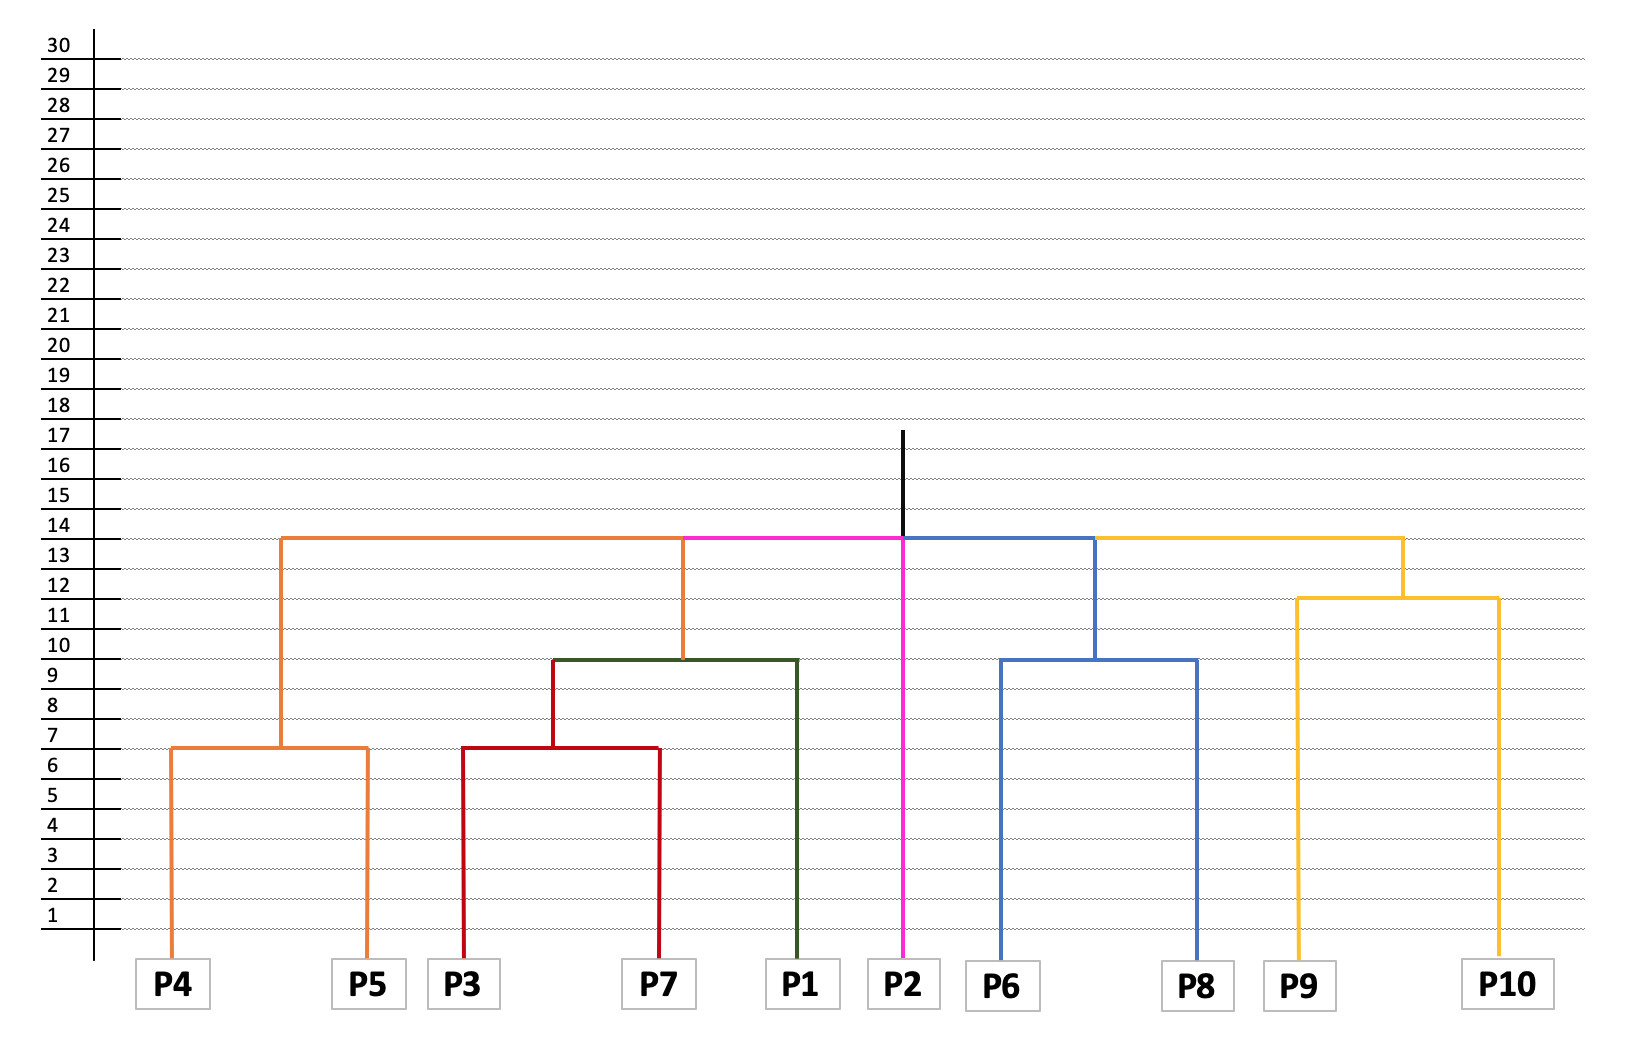
\includegraphics[width=17cm]{Dendrograma.png} 
    \end{figure}
  \end{center}
  

\newpage
\setcounter{section}{4}
\section{CAPÍTULO 05: CLASSIFICAÇÃO DE DADOS}
\subsection{EXERCÍCIOS CONCEITUAIS}
\subsubsection{Durante o desenvolvimento de um modelo de classificação a base de dados é dividida em dois conjuntos. Quais são estes conjuntos e qual é o propósito desta separação}
\textit{Resposta:} Os dois conjuntos são: treinamento e testes. Seu propósito é gerar modelos preditivos capazes de identificar classes ou valores de registros não rotulados com um resultado satisfatório. 

\subsubsection{Discuta por quê para bases de dados reais na maioria das vezes treinar um sistema preditivo até que o erro para os dados de treinamento seja zero não é aconselhável.}
\textit{Resposta:} Durante o processo de treinamento de modelos, mesmo com o desempenho cada vez melhor e a quantidade de erros possa estar decaindo, o desempenho de generalização pode começar a se deteriorar após determinado número de iterações. \\
O ideal é utilizar uma validação cruzada para interromper o treinamento para conseguir obter um melhor resultado.

\subsubsection{O que é a validação cruzada em k-pastas? Qual é a sua finalidade?}
\textit{Resposta:} A validação cruzada em k-pastas consiste em dividir a base de dados em k subconjuntos, sendo k –1 pastas para treinamento e 1 pasta para teste. Esse processo de treinamento e teste é repetido com todos os k subconjuntos, e a média dos desempenhos para as bases de treinamento e as bases de teste é adotada como indicador de qualidade do modelo. \\
A validação cruzada em k-pastas é bastante usual para se estimar o erro de generalização de preditores.


\subsubsection{O que é a matriz de confusão de um problema de classificação binária? Explique os quatro valores apresentados pela matriz.}
\textit{Resposta:} Matriz de confusão é uma forma de apresentar integralmente o desempenho de um algoritmo de classificação binária utilizando uma matriz que relaciona as classes desejadas com as classes preditas. \\
Essa matriz também é conhecida como \textit{matriz de contingência} ou \textit{matriz de erro} e na sua composição ela tem nas linhas os objetos nas classes originais e nas colunas os objetos nas classes preditas.

\begin{center}
  \begin{table}[H]
    \centering
      \begin{tabular}{ll|c|c|}
      \cline{3-4}
                                                                                      &                                                       & \multicolumn{2}{c|}{\cellcolor[HTML]{C0C0C0}Classe predita}         \\ \cline{3-4} 
                                                                                      &                                                       & \cellcolor[HTML]{C0C0C0}Positiva & \cellcolor[HTML]{C0C0C0}Negativa \\ \hline
      \multicolumn{1}{|c|}{\cellcolor[HTML]{C0C0C0}}                                  & \multicolumn{1}{c|}{\cellcolor[HTML]{C0C0C0}Positiva} & VP                               & FN                               \\ \cline{2-4} 
      \multicolumn{1}{|c|}{\multirow{-2}{*}{\cellcolor[HTML]{C0C0C0}Classe original}} & \multicolumn{1}{c|}{\cellcolor[HTML]{C0C0C0}Negativa} & FP                               & VN                               \\ \hline
    \end{tabular}
  \end{table}
\end{center}

Abaixo estão as explicações dos quatro valores apresentados na tabela.

\begin{itemize}
  \item \textbf{VP (verdadeiro positivo):} você previu positivo e é verdadeiro \\ Ex.: Você previu que uma mulher está grávida e ela realmente está.
  \item \textbf{VN (verdadeiro negativo):} você previu negativo e é verdadeiro \\ Ex.: Você previu que um homem não está grávido e ele realmente não está.
  \item \textbf{FP (falso positivo):} você previu positivo e é falso \\ Ex.: Você previu que um homem está grávido, mas na verdade ele não está.
  \item \textbf{FN (falso negativo):} você previu negativo e é falso \\ Ex.: Você previu que uma mulher não está grávida, mas na verdade ela está.
\end{itemize}
\newpage

\subsection{EXERCÍCIOS NUMÉRICOS}

\subsubsection{Utilizando a árvore de decisão para o conjunto de treinamento da base de dados Cogumelos, apresentada na Figura 5.19, extraia todas as regras de classificação para cogumelos venenosos.}
\begin{figure}[H]
  \centering 
  \includegraphics[width=10cm]{Figura-5-19.png} 
  \caption*{Figura 5.19}
\end{figure}

\textit{Resposta:} 
\begin{table}[H]
  \centering
  \begin{tabular}{|c|c|c|}
    \hline
    \rowcolor[HTML]{C0C0C0} 
    \textbf{Atributo} & \textbf{Valor} & \textbf{Classe} \\ \hline
    odor              & creosoto       & venenoso        \\ \hline
    odor              & peixe          & venenoso        \\ \hline
    odor              & podre          & venenoso        \\ \hline
    odor              & mofado         & venenoso        \\ \hline
    odor              & ácido          & venenoso        \\ \hline
    odor              & apimentado     & venenoso        \\ \hline
    cor do esporo     & verde          & venenoso        \\ \hline
    espaço da lamela  & fechado        & venenoso        \\ \hline
    população         & agrupada       & venenoso        \\ \hline
  \end{tabular}
\end{table}

\subsubsection{Considere o seguinte problema: Um determinado algoritmo é responsável por indicar se um paciente está doente ou não. Após a realização de um experimento com 150 pacientes, onde 30 estavam doentes, o algoritmo informou a existência de 28 doentes sendo que 8 destes estavam saudáveis. Calcule a taxa de verdadeiro positivo \textit{(TPR)}, a taxa de falso positivo \textit{(FPR)}, a acurácia  \textit{(ACC)}, e a precisão \textit{(Pr)}.}
\textit{Resposta:} 

\begin{center}
  \begin{table}[H]
    \centering
      \begin{tabular}{ll|c|c|}
      \cline{3-4}
                                                                                      &                                                       & \multicolumn{2}{c|}{\cellcolor[HTML]{C0C0C0}Classe predita}         \\ \cline{3-4} 
                                                                                      &                                                       & \cellcolor[HTML]{C0C0C0}Positiva & \cellcolor[HTML]{C0C0C0}Negativa \\ \hline
      \multicolumn{1}{|c|}{\cellcolor[HTML]{C0C0C0}}                                  & \multicolumn{1}{c|}{\cellcolor[HTML]{C0C0C0}Positiva} & 20                               & 10                               \\ \cline{2-4} 
      \multicolumn{1}{|c|}{\multirow{-2}{*}{\cellcolor[HTML]{C0C0C0}Classe original}} & \multicolumn{1}{c|}{\cellcolor[HTML]{C0C0C0}Negativa} & 8                                & 112                               \\ \hline
    \end{tabular}
  \end{table}
\end{center}

\textbf{Taxa de verdadeiro positivo (TVP):} 
\begin{center}
  $TVP = \dfrac{VP}{VP + FN} = $
  $\dfrac{20}{30} = 0.6666 \cdot 100 = 66.66\%$    
\end{center}

\textbf{Taxa de falso positivo (TFP):} 
\begin{center}
  $TFP = \dfrac{FP}{FP + VN} = $
  $\dfrac{8}{120} = 0.0666 \cdot 100 = 6,67\%$
\end{center}

\textbf{Acurácia (ACC):} 
\begin{center}
  $ACC = \dfrac{VP + VN}{VP+FP+VN+FN} = \dfrac{132}{150} = 0.88 \cdot 100 = 88\%$
\end{center}

\textbf{Precisão (PR):} 
\begin{center}
  $Pr = \dfrac{VP}{FP + VP} = \dfrac{20}{28} = 0.7143 \cdot 100 = 71.43\%$
\end{center}

\textbf{Conclusão:}
\begin{center}
  $\textit{TVP} = 66.66\%$ \\
  $\textit{TFP} = 6.67\%$ \\
  $\textit{ACC} = 88\%$ \\
  $\textit{Pr} = 71.43\%$
\end{center}

\subsubsection{Construa uma árvore de decisão para a base de dados abaixo.}
  \begin{figure}[H]
    \centering 
    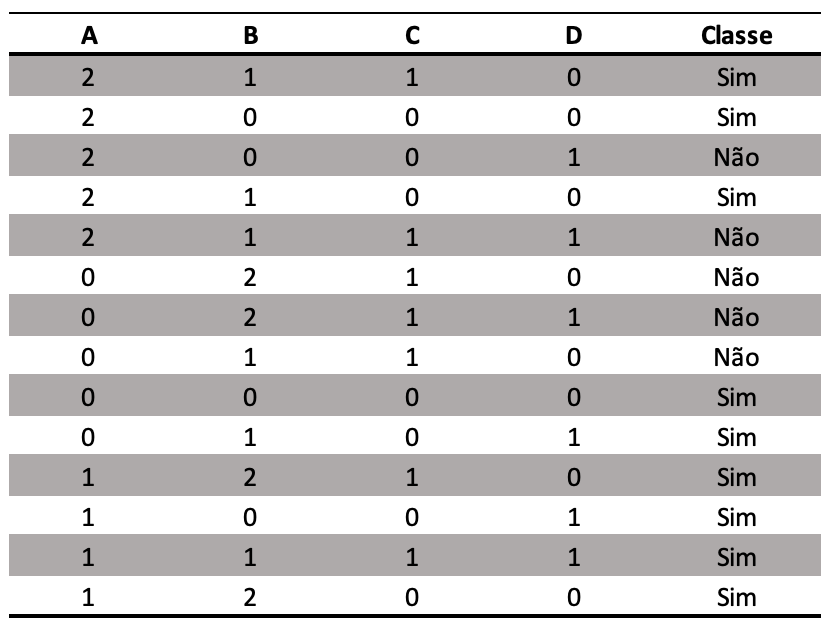
\includegraphics[width=8cm]{tab-5-2-3.png} 
  \end{figure}

\textit{Resposta:} 

\begin{figure}[H]
  \centering 
  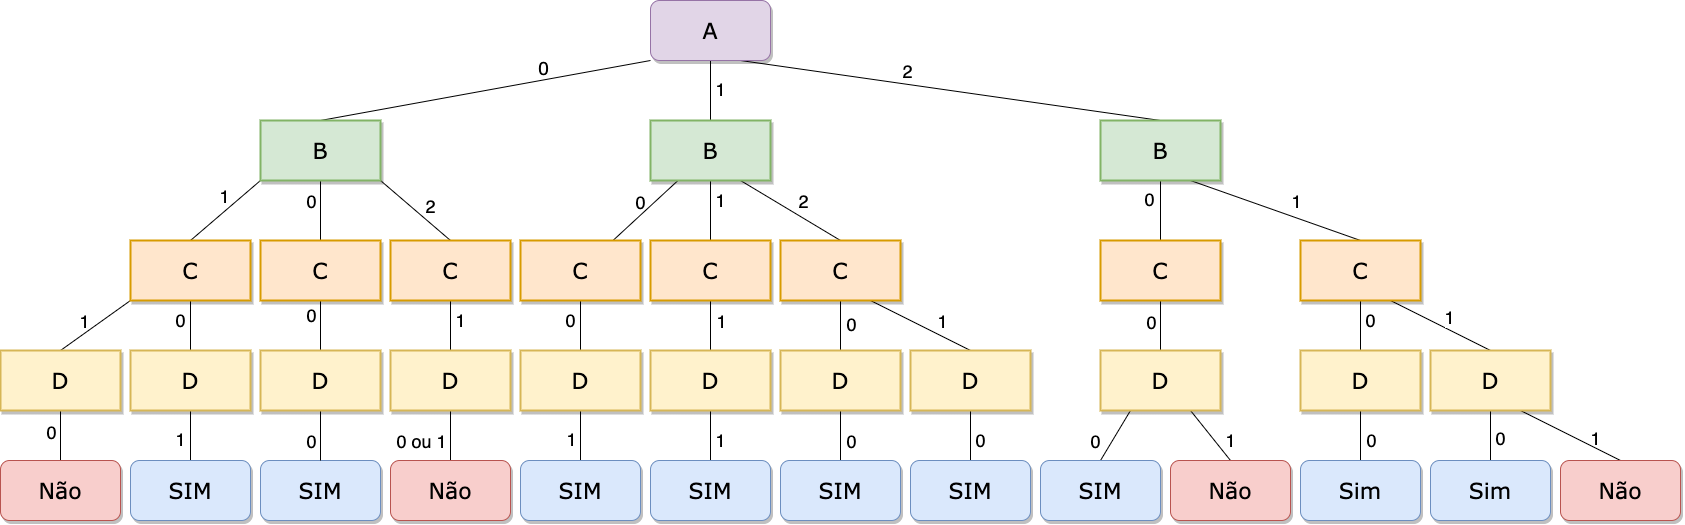
\includegraphics[width=17cm]{arvore-decisao.png} 
\end{figure}

\subsubsection{Aplique o classificador \textit{Naïve Bayes} na base de dados abaixo e determine o valor para classe \textbf{Jogar} dos seguintes objetos:}
\begin{enumerate}[label=\alph*]
    \item X = (Ensolarado, Branda, Alta, Não)
    \item Y = (Chuvoso, Fria, Alta, Sim)
    \item Z = (Ensolarado, Branda, Normal, Não)
    \item W = (Fechado , Fria, Normal, Sim)
\end{enumerate}

\begin{figure}[H]
    \centering 
    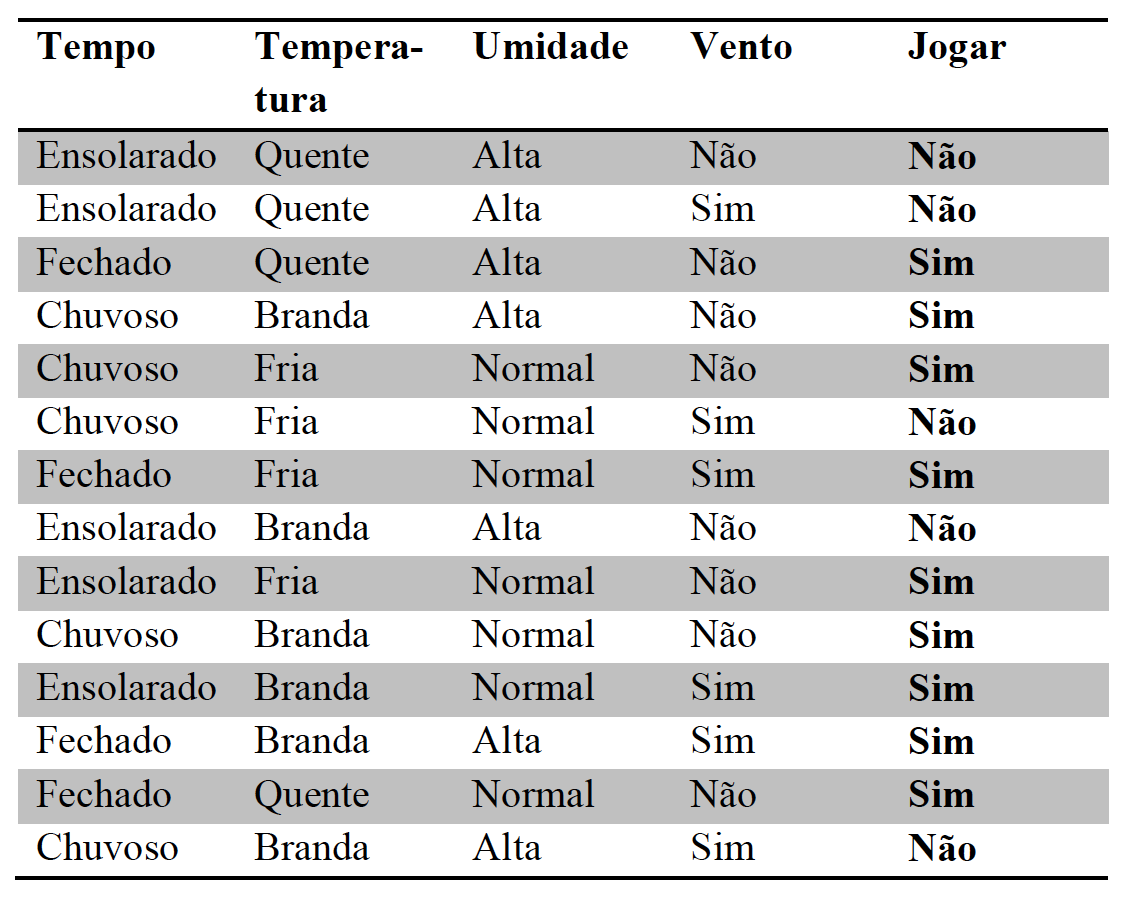
\includegraphics[width=8cm]{tab-5-2-4.png} 
  \end{figure}

\textit{Resposta:} 
\textbf{Teorema de Bayes:}
$P(C_i \mid x) = \dfrac{P(x \mid C_i)P(C_i)}{P(x)}$

\textbf{Probabilidade por atributo:}
  \begin{table}[H]
    \centering
    \begin{tabular}{cccc}
      \hline
      \rowcolor[HTML]{EFEFEF} 
      \multicolumn{1}{|c|}{\cellcolor[HTML]{EFEFEF}\textbf{Tempo}}       & \multicolumn{1}{c|}{\cellcolor[HTML]{EFEFEF}\textbf{Jogar = Sim}} & \multicolumn{1}{c|}{\cellcolor[HTML]{EFEFEF}\textbf{Jogar = Não}} & \multicolumn{1}{c|}{\cellcolor[HTML]{EFEFEF}\textbf{Total}} \\ \hline
      \multicolumn{1}{|c|}{Ensolarado}                                   & \multicolumn{1}{c|}{2/9 = 0.22}                                   & \multicolumn{1}{c|}{3/5 = 0.6}                                    & \multicolumn{1}{c|}{5/14 = 0.36}                            \\ \hline
      \multicolumn{1}{|c|}{Fechado}                                      & \multicolumn{1}{c|}{4/9 = 0.44}                                   & \multicolumn{1}{c|}{0/5 = 0}                                      & \multicolumn{1}{c|}{4/14 = 0.28}                            \\ \hline
      \multicolumn{1}{|c|}{Chuvoso}                                      & \multicolumn{1}{c|}{3/9 = 0.33}                                   & \multicolumn{1}{c|}{2/5 = 0.55}                                   & \multicolumn{1}{c|}{5/14 = 0.36}                            \\ \hline
      \multicolumn{1}{l}{}                                               & \multicolumn{1}{l}{}                                              & \multicolumn{1}{l}{}                                              & \multicolumn{1}{l}{}                                        \\ \hline
      \rowcolor[HTML]{EFEFEF} 
      \multicolumn{1}{|c|}{\cellcolor[HTML]{EFEFEF}\textbf{Temperatura}} & \multicolumn{1}{c|}{\cellcolor[HTML]{EFEFEF}\textbf{Jogar = Sim}} & \multicolumn{1}{c|}{\cellcolor[HTML]{EFEFEF}\textbf{Jogar = Não}} & \multicolumn{1}{c|}{\cellcolor[HTML]{EFEFEF}\textbf{Total}} \\ \hline
      \multicolumn{1}{|c|}{Quente}                                       & \multicolumn{1}{c|}{2/9 = 0.22}                                   & \multicolumn{1}{c|}{2/5 = 0.4}                                    & \multicolumn{1}{c|}{4/14 = 0.28}                            \\ \hline
      \multicolumn{1}{|c|}{Branda}                                       & \multicolumn{1}{c|}{4/9 = 0.44}                                   & \multicolumn{1}{c|}{2/5 = 0.4}                                    & \multicolumn{1}{c|}{6/14 = 0.43}                            \\ \hline
      \multicolumn{1}{|c|}{Fria}                                         & \multicolumn{1}{c|}{3/9 = 0.33}                                   & \multicolumn{1}{c|}{1/5 = 0.2}                                    & \multicolumn{1}{c|}{4/14 = 0.28}                            \\ \hline
      \multicolumn{1}{l}{}                                               & \multicolumn{1}{l}{}                                              & \multicolumn{1}{l}{}                                              & \multicolumn{1}{l}{}                                        \\ \hline
      \rowcolor[HTML]{EFEFEF} 
      \multicolumn{1}{|c|}{\cellcolor[HTML]{EFEFEF}\textbf{Umidade}}    & \multicolumn{1}{c|}{\cellcolor[HTML]{EFEFEF}\textbf{Jogar = Sim}} & \multicolumn{1}{c|}{\cellcolor[HTML]{EFEFEF}\textbf{Jogar = Não}} & \multicolumn{1}{c|}{\cellcolor[HTML]{EFEFEF}\textbf{Total}} \\ \hline
      \multicolumn{1}{|c|}{Alta}                                         & \multicolumn{1}{c|}{3/9 = 0.33}                                   & \multicolumn{1}{c|}{4/5 = 0.8}                                    & \multicolumn{1}{c|}{7/14 = 0.5}                             \\ \hline
      \multicolumn{1}{|c|}{Normal}                                       & \multicolumn{1}{c|}{6/9 = 0.67}                                   & \multicolumn{1}{c|}{1/5 = 0.2}                                    & \multicolumn{1}{c|}{7/15 = 0.5}                             \\ \hline
      \multicolumn{1}{l}{}                                               & \multicolumn{1}{l}{}                                              & \multicolumn{1}{l}{}                                              & \multicolumn{1}{l}{}                                        \\ \hline
      \rowcolor[HTML]{EFEFEF} 
      \multicolumn{1}{|c|}{\cellcolor[HTML]{EFEFEF}\textbf{Vento}}       & \multicolumn{1}{c|}{\cellcolor[HTML]{EFEFEF}\textbf{Joga = Sim}}  & \multicolumn{1}{c|}{\cellcolor[HTML]{EFEFEF}\textbf{Jogar = Não}} & \multicolumn{1}{c|}{\cellcolor[HTML]{EFEFEF}\textbf{Total}} \\ \hline
      \multicolumn{1}{|c|}{Sim}                                          & \multicolumn{1}{c|}{3/9 = 0.33}                                   & \multicolumn{1}{c|}{3/5 = 0.6}                                    & \multicolumn{1}{c|}{6/14 = 0.43}                            \\ \hline
      \multicolumn{1}{|c|}{Não}                                          & \multicolumn{1}{c|}{6/9 = 0.67}                                   & \multicolumn{1}{c|}{2/5 = 0.4}                                    & \multicolumn{1}{c|}{8/14 = 0.57}                            \\ \hline
    \end{tabular}
  \end{table}

  
  \begin{tabbing}
    \textbf{Probabilidade de Jogar (Sim/Não) $P(C)$:} 
    $P(Jogar=SIM) = \text{9/14} = 0.64$ \\
    $P(Jogar=NAO) = \text{5/14} = 0.36$ \\
  \end{tabbing}

  \textbf{\large Problema: a) - X = (Ensolarado, Branda, Alta, Não):}
  
  \begin{tabbing}
    \textbf{Probabilidade de Jogar=Sim por atributo:}\\
    $P(Tempo=Ensolarado \mid Jogar = Sim) =  0.22 $ \\
    $P(Temperatura=Branda \mid Jogar = Sim)  = 0.44 $ \\
    $P(Umidade=Alta \mid Jogar = Sim)  = 0.33 $ \\
    $P(Vento=Nao \mid Jogar = Sim) = 0.67 $ \\
    $P(Jogar=Sim) = 0.64$ \\
    $P(X \mid Jogar=Sim)P(Jogar=Sim) = 0.22 \cdot 0.44 \cdot 0.33 \cdot 0.67 \cdot 0.64 = 0.0137$ \\
  \end{tabbing}
  
  \begin{tabbing}
    \textbf{Probabilidade de Jogar=Nao por atributo:}\\
    $P(Tempo=Ensolarado \mid Jogar = Nao) =  0.6 $ \\
    $P(Temperatura=Branda \mid Jogar = Nao)  = 0.4 $ \\
    $P(Umidade=Alta \mid Jogar = Nao)  = 0.8 $ \\
    $P(Vento=Nao \mid Jogar = Nao) = 0.4 $ \\
    $P(Jogar=Nao) = 0.36$ \\
    $P(X \mid Jogar=Nao)P(Jogar=Nao) = 0.6 \cdot 0.4 \cdot 0.8 \cdot 0.4 \cdot 0.36 = 0.0276$ \\
  \end{tabbing}

  \begin{tabbing}
    \textbf{Probabilidade do total dos atributos:}\\
    $P(X) = P(Tempo=Ensolarado) \cdot P(Temperatura=Branda) \cdot P(Umidade=Alta) \cdot P(Vento=Nao)$ \\
    $P(X) = 0.36 \cdot 0.43 \cdot 0.5 \cdot 0.57$ \\
    $P(X) = 0.0441$  
  \end{tabbing}
  
  \begin{tabbing}
    \textbf{Probabilidade de Jogar:}\\
    $P(Jogar=Sim) \mid X) = \dfrac{0.0137}{0.0441} = 0.3106$ \\
    $P(Jogar=Nao) \mid X) = \dfrac{0.0276}{0.0441} = \textbf{0.6258}$
  \end{tabbing}

  \begin{tabbing}
    \textbf{Conclusão de X:}
    Probabilidade de Jogar = \textbf{NÃO}\\
  \end{tabbing}  

  \textbf{\large Problema: b) - Y = (Chuvoso, Fria, Alta, Sim):}
  
  \begin{tabbing}
    \textbf{Probabilidade de Jogar=Sim por atributo:}\\
    $P(Tempo=Chuvoso \mid Jogar = Sim) =  0.33 $ \\
    $P(Temperatura=Fria \mid Jogar = Sim)  = 0.33 $ \\
    $P(Umidade=Alta \mid Jogar = Sim)  = 0.33 $ \\
    $P(Vento=Sim \mid Jogar = Sim) = 0.33 $ \\
    $P(Jogar=Sim) = 0.64$ \\
    $P(Y \mid Jogar=Sim)P(Jogar=Sim) = 0.33 \cdot 0.33 \cdot 0.33 \cdot 0.33 \cdot 0.64 = 0.0076$ \\
  \end{tabbing}

  
  \begin{tabbing}
    \textbf{Probabilidade de Jogar=Nao por atributo:}\\
    $P(Tempo=Chuvoso \mid Jogar = Nao) =  0.6 $ \\
    $P(Temperatura=Fria \mid Jogar = Nao)  = 0.2 $ \\
    $P(Umidade=Alta \mid Jogar = Nao)  = 0.8 $ \\
    $P(Vento=Sim \mid Jogar = Nao) = 0.6 $ \\
    $P(Jogar=Nao) = 0.36$ \\
    $P(Y \mid Jogar=Nao)P(Jogar=Nao) = 0.6 \cdot 0.2 \cdot 0.8 \cdot 0.6 \cdot 0.36 = 0.0207$ \\
  \end{tabbing}

  
  \begin{tabbing}
    \textbf{Probabilidade do total dos atributos:}\\
    $P(Y) = P(Tempo=Chuvoso) \cdot P(Temperatura=Fria) \cdot P(Umidade=Alta) \cdot P(Vento=Sim)$ \\
    $P(Y) = 0.36 \cdot 0.28 \cdot 0.5 \cdot 0.43$ \\
    $P(Y) = 0.0217$  
  \end{tabbing}
  
  
  \begin{tabbing}
    \textbf{Probabilidade de Jogar:}\\
    $P(Jogar=Sim) \mid Y) = \dfrac{0.0076}{0.0217} = 0.3502$ \\
    $P(Jogar=Nao) \mid Y) = \dfrac{0.0207}{0.0217} = \textbf{0.9539}$
  \end{tabbing}

  \begin{tabbing}
    \textbf{Conclusão de Y:}
    Probabilidade de Jogar = \textbf{NÃO} \\
  \end{tabbing}

  \textbf{\large Problema: c) - Z = (Ensolarado, Branda, Normal, Não):}
  
  \begin{tabbing}
    \textbf{Probabilidade de Jogar=Sim por atributo:}\\
    $P(Tempo=Ensolarado \mid Jogar = Sim) =  0.22 $ \\
    $P(Temperatura=Branda \mid Jogar = Sim)  = 0.44 $ \\
    $P(Umidade=Normal \mid Jogar = Sim)  = 0.67 $ \\
    $P(Vento=Nao \mid Jogar = Sim) = 0.67 $ \\
    $P(Jogar=Sim) = 0.64$ \\
    $P(Z \mid Jogar=Sim)P(Jogar=Sim) = 0.22 \cdot 0.44 \cdot 0.67 \cdot 0.67 \cdot 0.64 = 0.0278$ \\
  \end{tabbing}

  \begin{tabbing}
    \textbf{Probabilidade de Jogar=Nao por atributo:}\\
    $P(Tempo=Ensolarado \mid Jogar = Nao) =  0.6 $ \\
    $P(Temperatura=Branda \mid Jogar = Nao)  = 0.4 $ \\
    $P(Umidade=Normal \mid Jogar = Nao)  = 0.2 $ \\
    $P(Vento=Nao \mid Jogar = Nao) = 0.4 $ \\
    $P(Jogar=Nao) = 0.36$ \\
    $P(Z \mid Jogar=Nao)P(Jogar=Nao) = 0.6 \cdot 0.4 \cdot 0.2 \cdot 0.4 \cdot 0.36 = 0.0069$ \\
  \end{tabbing}

  \begin{tabbing}
    \textbf{Probabilidade do total dos atributos:}\\
    $P(Z) = P(Tempo=Ensolarado) \cdot P(Temperatura=Branda) \cdot P(Umidade=Normal) \cdot P(Vento=Nao)$ \\
    $P(Z) = 0.36 \cdot 0.43 \cdot 0.5 \cdot 0.57$ \\
    $P(Z) = 0.0441$  
  \end{tabbing}
  
  \begin{tabbing}
    \textbf{Probabilidade de Jogar:}\\
    $P(Jogar=Sim) \mid Z) = \dfrac{0.0278}{0.0441} = \textbf{0.6303}$ \\
    $P(Jogar=Nao) \mid Z) = \dfrac{0.0069}{0.0441} = 0.1564$
  \end{tabbing}

  \begin{tabbing}
    \textbf{Conclusão de Z:}
    Probabilidade de Jogar = \textbf{SIM} \\
  \end{tabbing} 

  \textbf{\large Problema: d) - W = (Fechado, Fria, Normal, Sim):}
  
  \begin{tabbing}
    \textbf{Probabilidade de Jogar=Sim por atributo:}\\
    $P(Tempo=Fechado \mid Jogar = Sim) =  0.44 $ \\
    $P(Temperatura=Fria \mid Jogar = Sim)  = 0.33 $ \\
    $P(Umidade=Normal \mid Jogar = Sim)  = 0.67 $ \\
    $P(Vento=Sim \mid Jogar = Sim) = 0.33 $ \\
    $P(Jogar=Sim) = 0.64$ \\
    $P(W \mid Jogar=Sim)P(Jogar=Sim) = 0.44 \cdot 0.33 \cdot 0.67 \cdot 0.33 \cdot 0.64 = 0.0109$ \\
  \end{tabbing}

  \begin{tabbing}
    \textbf{Probabilidade de Jogar=Nao por atributo:}\\
    $P(Tempo=Fechado \mid Jogar = Nao) =  0 $ \\
    $P(Temperatura=Fria \mid Jogar = Nao)  = 0.33 $ \\
    $P(Umidade=Normal \mid Jogar = Nao)  = 0.2 $ \\
    $P(Vento=Sim \mid Jogar = Nao) = 0.6 $ \\
    $P(Jogar=Nao) = 0.36$ \\
    $P(W \mid Jogar=Nao)P(Jogar=Nao) = 0 \cdot 0.33 \cdot 0.2 \cdot 0.6 \cdot 0.36 = 0$ \\
  \end{tabbing}

  \begin{tabbing}
    \textbf{Probabilidade do total dos atributos:}\\
    $P(W) = P(Tempo=Fechado) \cdot P(Temperatura=Fria) \cdot P(Umidade=Normal) \cdot P(Vento=Sim)$ \\
    $P(W) = 0.28 \cdot 0.28 \cdot 0.5 \cdot 0.43$ \\
    $P(W) = 0.0168$  
  \end{tabbing}
  
  \begin{tabbing}
    \textbf{Probabilidade de Jogar:}\\
    $P(Jogar=Sim) \mid W) = \dfrac{0.0109}{0.0168} = \textbf{0.6488}$ \\
    $P(Jogar=Nao) \mid W) = \dfrac{0}{0.0168} = 0$
  \end{tabbing}

  \begin{tabbing}
    \textbf{Conclusão de W:}
    Probabilidade de Jogar = \textbf{SIM} \\
  \end{tabbing}
\end{document}